\documentclass[tikz,border=6pt]{standalone}
\usepackage[T1]{fontenc}
\usepackage{lmodern}
\usepackage{amssymb}
\usetikzlibrary{positioning,arrows.meta,calc}

\newcommand{\Nat}{$\mathbb{N}$}

\begin{document}
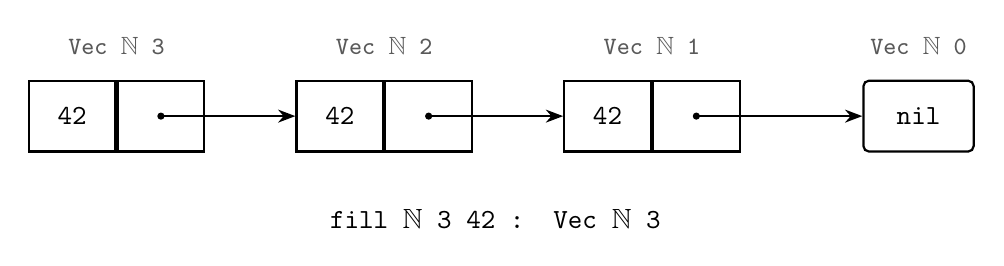
\begin{tikzpicture}[
    >={Stealth[length=2.2mm]},
    cell/.style={draw, thick, minimum width=11mm, minimum height=9mm, font=\ttfamily},
    nil/.style={draw, thick, rounded corners=2pt, minimum width=14mm,
                minimum height=9mm, font=\ttfamily},
    ty/.style={font=\ttfamily\small, text=gray!70!black},
  ]
  \def\dx{3.4}

  \foreach \i/\n in {0/3, 1/2, 2/1} {
    \node[cell] (h\i) at (\i*\dx, 0) {42};
    \node[cell, right=0mm of h\i] (t\i) {};
    \fill ($(t\i.center)$) circle (1.3pt);
    \node[ty, above=2mm of $(h\i.north east)$] {Vec \Nat{} \n};
  }
  \node[nil] (nil) at (3*\dx+0.55, 0) {nil};
  \node[ty, above=2mm of nil] {Vec \Nat{} 0};

  \draw[->, thick] (t0.center) -- (h1.west);
  \draw[->, thick] (t1.center) -- (h2.west);
  \draw[->, thick] (t2.center) -- (nil.west);

  \node[font=\ttfamily, below=6mm of $(h0.south)!0.5!(nil.south)$]
    {fill \Nat{} 3 42 : Vec \Nat{} 3};
\end{tikzpicture}
\end{document}
